\section{Risk-Based Stochastic Capital Budgeting using Conditional Value-at-Risk}
\label{sec:CVaR}

Value-at-Risk (VaR) is currently used by finance businesses to indicate the percentiles
of loss distributions. For instance, $95\%$-VaR is an upper estimate of losses which
is exceeded with $5\%$ probability. The popularity of VaR is mostly related to a simple
and easy to understand representation of high losses. However, VaR may have undesirable
mathematical characteristics such as a lack of subadditivity and convexity~\cite{ThinkingCoherently,CoherentMeasureRisk} .
Another alternative percentile risk measure is called Conditional Value-at-Risk (CVaR),
which has more attractive properties than VaR, such as sub-additive and convex.
CVaR also called mean excess loss, mean shortfall, or tail VaR, is defined as the
expected loss exceeding VaR. In general, CVaR is the weighted average of VaR and
losses exceeding VaR. In this section, we will focus on using CVaR for capital
budgeting problem.

\subsection{Definitions of VaR and CVaR}
\label{definitionCVaR}
Let $X$ be a random variable with a cumulative distribution function
$F(z) = P{X\le z}$. It can be useful to think of $X$ as a ``loss'' or more generally
a variable such that large values need to be avoid. The VaR of $X$ with confidence level
$\alpha$ (e.g., $\alpha = 0.9$ is:

\begin{equation}
VaR_\alpha (X) = \min {z|F_X(z)\ge \alpha}
\end{equation}

which is equivalent to $VaR_\alpha (X) = F_{X}^{-1}(\alpha)$ if $X$ is a continuous
random variable. By this definition, $VaR_\alpha (X)$ is a (lower) $\alpha$-percentile
of the random variable $X$. An alternative measure of risk is CVaR. Here, $CVaR_\alpha (X)$
is the conditional expectation of $X$ given that $X \ge VaR_\alpha (X)$.
Figure~\ref{fig:CVaR} shows the relationship between these two measures of risk.

\begin{figure}
    \centering
    \centerline{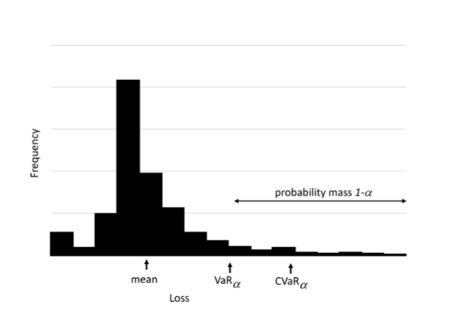
\includegraphics[scale=0.5]{CVaR.jpg}}
    \caption{Relationship between value-at-risk and conditional value-at-risk.}
    \label{fig:CVaR}
\end{figure}

The typical definition of $CVaR_\alpha (X)$ is $CVaR_\alpha (X) = E{X|X > VaR_\alpha (X)}$.
There are alternative ways to define this measure, which are mathematically equivalent.
Rockafellar and Uryasev in~\cite{OptCVaR} (see also~\cite{RemarksCVaR}) defines CVaR as:

\begin{equation}
CVaR_\alpha (X) = \min_u {u + 1/(1-\alpha) E[X-u]^+}
\end{equation}

where $[X-u] = \max (X - u, 0)$. Here, variable $u$ is simply an auxiliary decision
variable whose optimal value turns out to be $CVaR_\alpha (X)$. The above definition
is particularly useful for computation in the context of optimization.

Researchers have argued for using CVaR over VaR as a measure of risk. Theoretically,
CVaR satisfies the assumptions of a so-called coherent risk measure, and VaR does not.
In simpler terms, minimizing VaR is concerned with the numerical value of the 95-th
percentile (say) of the loss, but it does not care about the magnitude of larger losses.
CVaR takes these magnitudes into account.

\subsection{CVaR in Capital Budgeting}
\label{CVaRCapitalBudgeting}
In this section, an explicit risk measure is constructed using a weighted
combination of expectation and CVaR. This approach allows us to parametrically
vary the weight on maximizing expected NPV versus penalizing solutions that yield
low-NPV scenarios, and we denote the weight by $\lambda$ with $0 \le \lambda \le 1$.
Let $NPV(s,\xi)$ denote the net present value under a prioritization decision
specified by decision $s$, and under a realization of the budget and profit of
each project, denoted by $\xi$. Then we seek to solve the following optimization
model:

\begin{equation}
\max_{s\in S} (1-\lambda)E[NPV(s, \xi)] - \lambda CVaR_\alpha [-NPV(s, \xi)]
\end{equation}

When $\lambda = 0$ the model reduces to stochastic optimization model as
discussed in Section~\ref{sec:StochasticCapitalBudgeting}; i.e., we seek
a prioritization decision, $s$, to maximize expected NPV, where ``$s \in S$''
simply indicates the constraints that a prioritized solution must satisfy.
$CVaR_\alpha [X]$ is typically applied to a random variable, $X$, which
represents a loss; i.e., we seek to avoid large values of $X$. In this
context, let $VaR_\alpha [X]$ denote the $\alpha$-level quantile of $X$.
Thus, if $\alpha = 0.75$ then $VaR_0.75 [X]$ is the value such that $75\%$
of the realizations of $X$ have lower values of loss. Suppose for simplicity
that $NPV(s, \xi)$ values are positive. Large values of $NPV(s, \xi)$ are
good, and hence large values of $-NPV(s, \xi)$ (i.e., those closer to zero)
are bad. Using the definition of $CVaR_\alpha [X] = E[X|X > VaR_\alpha [X]]$
we thus have that the conditional value-at-risk is the expected value of loss,
given that the loss exceeds a certain percentile. So, when $\lambda = 1$ we
seek to minimize the expected value of NPV given that they fall below a
threshold. More generally, values of $\lambda$ between 0 and 1 seek a trade-off
between reward and risk, captured by expected NPV and CVaR, respectively.

The full mathematical optimization model of CVaR for capital budgeting problem
is as follows:

\begin{subequations}\label{fullCVaR}
\begin{eqnarray}
& & \max_{x, y, \nu, u} (1-\lambda) \sum _{ \omega  \in  \Omega }^{}q^{ \omega } \sum _{i \in I}^{} \sum _{j \in J_{i}}^{}a_{ij}^{ \omega }x_{ij}^{ \omega } - \lambda[u+1/(1-\alpha)\sum_{\omega \in \Omega} q^\omega \nu^\omega] \\
& & \nu^\omega \ge - \sum _{i \in I}^{} \sum _{j \in J_{i}}^{}a_{ij}^{ \omega }x_{ij}^{ \omega } - u, \omega \in \Omega \\
& & y_{ii^{'}}+y_{i^{'}i} \geq 1,~ i<i^{'}\text{, i, }i^{'} \in I \\
& & \sum_{j=1}^{J_i} x_{ij}^\omega \geq \sum_{j=1}^{J_i} x_{i'j}^\omega + y_{ii'} -1,~ i \neq i^{'}\text{, i, }i^{'} \in I,  \omega  \in  \Omega \\
& & \sum _{i \in I}^{} \sum _{j \in J_{i}}^{}\text{~ c}_{ijkt}^{ \omega }x_{ij}^{ \omega }~  \leq  b_{kt}^{ \omega },~ k \in K, t \in T,  \omega  \in  \Omega \\
& & \sum_{j\in J_i} x_{ij}^{ \omega } \leq 1,~ i \in I, \omega  \in  \Omega \\
& & y_{ii'}, x_{ij}^\omega \in {0, 1} \\
& & \nu^\omega \ge 0, \omega \in \Omega
\end{eqnarray}
\end{subequations}

\subsection{LOGOS Settings for CVaR Problems}
\label{subsec:CVaRSettings}
CVaR approach is an extension for stochastic optimization approach discussed in
Section~\ref{sec:StochasticCapitalBudgeting}. Both of them share the same input
structures except the \xmlNode{Settings} block. In both cases, the user need to
specify a collection of scenarios via \xmlNode{Uncertainties} block. The
\xmlNode{problem\_type} within \xmlNode{Settings} block is used to select the
type of CVaR problems. The currently available CVaR problem types are:
\xmlString{cvarskp}, \xmlString{cvarmkp}, and \xmlString{cvarmckp}. The user can
use \xmlNode{risk\_aversion} (i.e. $\lambda$) and \xmlNode{confidence\_level}
(i.e., $\alpha$) to control CVaR problem.

Example LOGOS input XML for CVaR:
\begin{lstlisting}[style=XML]
<Settings>
<Logos>
  <solver>cbc</solver>
  <solverOptions>
    <StochSolver>EF</StochSolver>
    <risk_aversion>0.1</risk_aversion>
    <confidence_level>0.95</confidence_level>
  </solverOptions>
  <sense>maximize</sense>
  <problem_type>cvarskp</problem_type>
</Settings>
</Logos>
\end{lstlisting}


\subsection{CVaR for Single Knapsack Problem}
\label{subsec:CVaR_SKP}

\vst \noi {\em Model Formulation:}
\begin{subequations}\label{CVaRSimpleKP}
\begin{eqnarray}
& & \max_{x, y, \nu, u} (1-\lambda)  \sum _{ \omega  \in  \Omega }^{}q^{ \omega } \sum _{i \in I}^{} a_{i}^{ \omega }x_{i}^{ \omega } - \lambda[u+1/(1-\alpha)\sum_{\omega \in \Omega} q^\omega \nu^\omega] \\
& & \nu^\omega \ge - \sum _{i \in I}^{} a_{i}^{ \omega }x_{i}^{ \omega } - u, \omega \in \Omega \\
& & \sum_{i \in I} c_{i}^\omega x_{i}^\omega \leq b^\omega, \omega \in \Omega\\
& & y_{ii'} + y_{i'i} \geq 1, i<i'  \\
& & x_{i}^\omega \geq x_{i'}^\omega + y_{ii'}-1, i\neq i' \\
& & x_{i}^\omega, y_{ii'}^\omega \in {0, 1} \\
& & \nu^\omega \ge 0, \omega \in \Omega, \lambda \in [0, 1]
\end{eqnarray}
\end{subequations}

See next section~\ref{subsec:CVaR_DKP} for the example of LOGOS input file, since multi-dimensional Knapsack problem
is just a simple extension of a single-dimensional Knapsack problem, and both of them belong to the same
\xmlNode{problem\_type}: \xmlString{cvarskp}.


\subsection{CVaR for Multi-Dimensional Knapsack Problem}
\label{subsec:CVaR_DKP}

\vst \noi {\em Model Formulation:}
\begin{subequations}\label{CVaRMultiDKP}
\begin{eqnarray}
& & \max_{x, y, \nu, u} (1-\lambda)  \sum _{ \omega  \in  \Omega }^{}q^{ \omega } \sum _{i \in I}^{} a_{i}^{ \omega }x_{i}^{ \omega } - \lambda[u+1/(1-\alpha)\sum_{\omega \in \Omega} q^\omega \nu^\omega] \\
& & \nu^\omega \ge - \sum _{i \in I}^{} a_{i}^{ \omega }x_{i}^{ \omega } - u, \omega \in \Omega \\
& & \sum_{i \in I} c_{it}^\omega x_{i}^\omega \leq b_{t}^\omega, t\in T \\
& & y_{ii'} + y_{i'i} \geq 1, i<i'  \\
& & x_{i}^\omega \geq x_{i'}^\omega + y_{ii'}-1, i\neq i' \\
& & x_{i}^\omega, y_{ii'}^\omega \in {0, 1} \\
& & \nu^\omega \ge 0, \omega \in \Omega, \lambda \in [0, 1]
\end{eqnarray}
\end{subequations}

Example LOGOS input XML:
\begin{lstlisting}[style=XML]
<Logos>
  <Sets>
    <investments>
      1,2,3,4,5,6,7,8,9,10,11,12,13,14,15,16
    </investments>
    <time_periods>
      1,2,3,4,5
    </time_periods>
  </Sets>

  <Parameters>
    <net_present_values index="investments">
      2.315,0.824,22.459,60.589,0.667,5.173,4.003,0.582,0.122,
      -2.870,-0.102,-0.278,-0.322,-3.996,-0.246,-20.155
    </net_present_values>
    <costs index="investments, time_periods">
      0.219,0.257,0.085,0.0,0.0,
      0.0,0.0,0.122,0.103,0.013,
      5.044,1.839,0.0,0.0,0.0,
      6.74,6.134,10.442,0.0,0.0,
      0.425,0.0,0.0,0.0,0.0,
      2.125,2.122,0.0,0.0,0.0,
      2.387,0.19,0.012,2.383,0.192,
      0.0,0.95,0.0,0.0,0.0,
      0.03,0.03,0.688,0.0,0.0,
      0,0.2,0.763,0.739,2.539,
      0.081,0.032,0,0,0,
      0.3,0,0,0,0,
      0.347,0,0,0,0,
      4.025,0.297,0,0,0,
      0.095,0.095,0.095,0,0,
      5.487,5.664,0.5,6.803,6.778
    </costs>
    <available_capitals index="time_periods">
      18,18,18,18,18
    </available_capitals>
  </Parameters>

  <Uncertainties>
    <available_capitals>
      <totalScenarios>10</totalScenarios>
      <probabilities>
        0.012, 0.019, 0.032, 0.052, 0.086, 0.142, 0.235, 0.188, 0.141, 0.093
      </probabilities>
      <scenarios>
        11, 11, 11, 11, 11,
        12, 12, 12, 12, 12,
        13, 13, 13, 13, 13,
        14, 14, 14, 14, 14,
        15, 15, 15, 15, 15,
        16, 16, 16, 16, 16,
        17, 17, 17, 17, 17,
        18, 18, 18, 18, 18,
        19, 19, 19, 19, 19,
        20, 20, 20, 20, 20
      </scenarios>
    </available_capitals>
  </Uncertainties>

  <Settings>
    <mandatory>10,11,12,13,14,15,16</mandatory>
    <solver>cbc</solver>
    <solverOptions>
      <StochSolver>EF</StochSolver>
      <!-- lambda for risk aversion -->
      <risk_aversion>0.1</risk_aversion>
      <!-- confidence level -->
      <confidence_level>0.95</confidence_level>
    </solverOptions>
    <sense>maximize</sense>
    <problem_type>cvarskp</problem_type>
  </Settings>
</Logos>
\end{lstlisting}


\subsection{CVaR for Multiple Knapsack Problem}
\label{subsec:CVaR_MKP}

\vst \noi {\em Model Formulation:}
\begin{subequations}\label{CVaRMKP}
\begin{eqnarray}
& & \max_{x, y, \nu, u} (1-\lambda)  \sum _{ \omega  \in  \Omega }^{}q^{ \omega } \sum_{m\in M} \sum _{i \in I}^{} a_{i}^{ \omega }x_{i, m}^{ \omega } - \lambda[u+1/(1-\alpha)\sum_{\omega \in \Omega} q^\omega \nu^\omega] \\
& & \nu^\omega \ge - \sum_{m\in M} \sum _{i \in I}^{} a_{i}^{ \omega }x_{i, m}^{ \omega } - u, \omega \in \Omega \\
& & \sum _{i \in I}^{} c_{i}^{ \omega }x_{im}^{ \omega }~  \leq  b_{m}^{ \omega },~ m \in M,  \omega  \in  \Omega \\
& & y_{ii'} + y_{i'i} \geq 1, i<i'  \\
& & \sum_{m=1}^{M} x_{im}^\omega \geq \sum_{m=1}^{M} x_{i'm}^\omega + y_{ii'} -1,~ i \neq i^{'}\text{, i, }i^{'} \in I,  \omega  \in  \Omega \\
& & \sum_{m=1}^{M} x_{im}^\omega \leq 1 \\
& & x_{im}^\omega, y_{ii'}^\omega \in {0, 1} \\
& & \nu^\omega \ge 0, \omega \in \Omega, \lambda \in [0, 1]
\end{eqnarray}
\end{subequations}

Example LOGOS input XML:
\begin{lstlisting}[style=XML]
<Logos>
  <Sets>
    <investments>
      1,2,3,4,5,6,7,8,9,10
    </investments>
    <capitals>
      unit_1, unit_2
    </capitals>
  </Sets>

  <Parameters>
    <net_present_values index="investments">
      78, 35, 89, 36, 94, 75, 74, 79, 80, 16
    </net_present_values>
    <costs index="investments">
      18, 9, 23, 20, 59, 61, 70, 75, 76, 30
    </costs>
    <available_capitals index="capitals">
      103, 156
    </available_capitals>
  </Parameters>

  <Uncertainties>
    <available_capitals>
      <totalScenarios>10</totalScenarios>
      <probabilities>
        0.1 0.1 0.1 0.1 0.1 0.1 0.1 0.1 0.1 0.1
      </probabilities>
      <scenarios>
        101, 154,
        102, 155,
        103, 156,
        104, 157,
        105, 158,
        106, 159,
        107, 160,
        108, 161,
        109, 162,
        110, 163
      </scenarios>
    </available_capitals>
  </Uncertainties>

  <Settings>
    <solver>cbc</solver>
    <solverOptions>
      <StochSolver>EF</StochSolver>
      <risk_aversion>1.0</risk_aversion>
      <confidence_level>0.95</confidence_level>
    </solverOptions>
    <sense>maximize</sense>
    <problem_type>cvarmkp</problem_type>
  </Settings>
</Logos>
\end{lstlisting}


\subsection{CVaR for Multiple-Choice Knapsack Problem}
\label{subsec:CVaR_MCKP}

\vst \noi {\em Model Formulation:}
\begin{subequations}\label{CVaRMCKP}
\begin{eqnarray}
& & \max_{x, y, \nu, u} (1-\lambda)  \sum _{ \omega  \in  \Omega }^{}q^{ \omega } \sum_{j\in J_i} \sum _{i \in I}^{} a_{ij}^{ \omega }x_{ij}^{ \omega } - \lambda[u+1/(1-\alpha)\sum_{\omega \in \Omega} q^\omega \nu^\omega] \\
& & \nu^\omega \ge - \sum_{j\in J_i} \sum _{i \in I}^{} a_{ij}^{ \omega }x_{ij}^{ \omega } - u, \omega \in \Omega \\
& & \sum _{i \in I}^{} \sum _{j \in J_{i}}^{}\text{~ c}_{ijkt}^{ \omega }x_{ij}^{ \omega }~  \leq  b_{kt}^{ \omega },~ k \in K, t \in T,  \omega  \in  \Omega \\
& & y_{ii'} + y_{i'i} \geq 1, i<i'  \\
& & \sum_{j=1}^{J_i - 1} x_{ij}^\omega \geq \sum_{j=1}^{J_i - 1} x_{i'j}^\omega + y_{ii'} -1,~ i \neq i^{'}\text{, i, }i^{'} \in I,  \omega  \in  \Omega, and i \neq i' \\
& & \sum_{j=1}^{J_i} x_{ij}^\omega = 1 \\
& & x_{i,j}^\omega, y_{ii'}^\omega \in {0, 1} \\
& & \nu^\omega \ge 0, \omega \in \Omega, \lambda \in [0, 1]
\end{eqnarray}
\end{subequations}

Example LOGOS input XML:
\begin{lstlisting}[style=XML]
<Logos>
  <Sets>
    <investments>
      1, 2, 3, 4, 5, 6, 7, 8, 9, 10, 11, 12, 13, 14, 15, 16, 17
    </investments>
    <options index='investments'>
      1;
      1;
      1;
      1,2,3;
      1,2,3,4;
      1,2,3,4,5,6,7;
      1;
      1;
      1;
      1;
      1;
      1;
      1;
      1;
      1;
      1;
      1
    </options>
  </Sets>

  <Parameters>
    <net_present_values index='options'>
      2.046
      2.679
      2.489
      2.61
      2.313
      1.02
      3.013
      2.55
      3.351
      3.423
      3.781
      2.525
      2.169
      2.267
      2.747
      4.309
      6.452
      2.849
      7.945
      2.538
      1.761
      3.002
      3.449
      2.865
      3.999
      2.283
      0.9
      8.608
    </net_present_values>
    <costs index='options'>
      36538462
      83849038
      4615385
      2788461538
      2692307692
      5480769231
      1634615385
      2981730768
      7211538462
      9038461538
      649038462
      650000000
      216346154
      212500000
      3076923077
      3942307692
      1144230769
      675721154
      1442307692
      99711538
      4807692
      123076923
      138461538
      86538462
      108653846
      75092404
      6413462
      147932692
    </costs>
    <available_capitals>
      15E9
    </available_capitals>
  </Parameters>

  <Uncertainties>
    <available_capitals>
      <totalScenarios>3</totalScenarios>
      <probabilities>
        0.2,0.6,0.2
      </probabilities>
      <scenarios>
        5E9,10E9,15E9
      </scenarios>
    </available_capitals>
  </Uncertainties>

  <Settings>
    <solver>glpk</solver>
    <solverOptions>
      <StochSolver>EF</StochSolver>
      <risk_aversion>0.1</risk_aversion>
      <confidence_level>0.95</confidence_level>
    </solverOptions>
    <sense>maximize</sense>
    <problem_type>cvarmckp</problem_type>
  </Settings>
</Logos>
\end{lstlisting}
